\documentclass[aspectratio=169,12pt,t]{beamer}

% --- Theme: Metropolis (modern, clean) ---
\usetheme[progressbar=frametitle,numbering=fraction,block=fill]{metropolis}

% --- Fira Sans font (install texlive-fonts-extra if missing) ---
\IfFileExists{FiraSans.sty}{\usepackage[sfdefault]{FiraSans}}{}

% --- Light background with warm accent ---
\definecolor{mDarkTeal}{RGB}{35,55,59}
\definecolor{mLightBrown}{RGB}{235,228,216}
\definecolor{mAccent}{RGB}{140,70,20}

\setbeamercolor{normal text}{fg=mDarkTeal,bg=white}
\setbeamercolor{alerted text}{fg=mAccent}
\setbeamercolor{frametitle}{bg=mDarkTeal,fg=white}
\setbeamercolor{progress bar}{fg=mAccent,bg=mLightBrown}
\setbeamercolor{title separator}{fg=mAccent}
\setbeamercolor{progress bar in head/foot}{fg=mAccent,bg=mLightBrown}
\setbeamercolor{progress bar in section page}{fg=mAccent,bg=mLightBrown}

% --- Packages ---
\usepackage[utf8]{inputenc}
\usepackage{amsmath,amssymb,amsthm}
\usepackage{mathrsfs}
\usepackage{tikz}
\usetikzlibrary{arrows.meta,positioning,calc,decorations.pathreplacing,shapes,patterns}
\usetikzlibrary{shadows.blur,backgrounds,fadings}
\usepackage{pgfplots}
\pgfplotsset{compat=1.18}

% --- Shared diagram styling (consistent, polished look across all figures) ---
\tikzset{
  setblob/.style={line width=1pt, rounded corners,
    blur shadow={shadow blur steps=8, shadow opacity=22,
                 shadow xshift=0pt, shadow yshift=-1.4pt}},
  blobblue/.style={setblob, draw=defcolor, fill=defcolor!10},
  blobred/.style={setblob, draw=thmcolor, fill=thmcolor!10},
  blobamber/.style={setblob, draw=excolor, fill=excolor!12},
  mapf/.style={-{Stealth[length=3mm,width=2.4mm]}, line width=1.2pt, mAccent},
  axisln/.style={-{Stealth[length=2.6mm]}, line width=0.8pt, gray!75},
  curveln/.style={line width=1.5pt, line cap=round, line join=round},
  projln/.style={dash pattern=on 2.6pt off 2pt, line width=0.7pt},
}
% point marker with a white halo: \dotpt{color}{(coord)}
\newcommand{\dotpt}[2]{%
  \fill[white] #2 circle (3.4pt);
  \fill[#1] #2 circle (2.2pt);
}
% open point marker: \opendot{color}{(coord)}
\newcommand{\opendot}[2]{%
  \fill[white] #2 circle (3.4pt);
  \draw[#1, line width=1.1pt] #2 circle (2.4pt);
}
% soft rounded background panel for inset plots
\tikzset{panel/.style={rounded corners=5pt, draw=mDarkTeal!14, line width=0.8pt,
  fill=mDarkTeal!4,
  blur shadow={shadow blur steps=8, shadow opacity=13,
               shadow xshift=0pt, shadow yshift=-1.3pt}}}
% small sequence-point marker: \seqdot{color}{(coord)}
\newcommand{\seqdot}[2]{\fill[#1] #2 circle (1.5pt);}

% --- Semi-transparent white highlight for text on top of background images ---
\usepackage[most]{tcolorbox}

% Inline highlight: \hl{short text}
\newtcbox{\hl}{%
  nobeforeafter, tcbox raise base,
  colback=white, opacityback=0.6,
  colframe=white, opacityframe=0,
  sharp corners, boxsep=2pt, left=3pt, right=3pt, top=2pt, bottom=2pt%
}

% Block highlight: \begin{hlbox} ... \end{hlbox}  (multi-line, paragraphs, itemize)
\newtcolorbox{hlbox}[1][]{%
  enhanced, breakable,
  colback=white, opacityback=0.6,
  colframe=white, opacityframe=0,
  boxsep=3pt, left=6pt, right=6pt, top=4pt, bottom=4pt,
  sharp corners,
  {#1}%
}

% --- Custom colors for content types ---
\definecolor{defcolor}{RGB}{25,85,120}
\definecolor{thmcolor}{RGB}{140,35,35}
\definecolor{proofcolor}{RGB}{35,100,50}
\definecolor{excolor}{RGB}{140,75,10}
\definecolor{remcolor}{RGB}{90,90,90}

% --- Beamer blocks for mathematical content types (semi-transparent) ---
\tcbset{hlblockbase/.style={
  enhanced, breakable,
  coltitle=white, fonttitle=\bfseries,
  opacitybacktitle=0.8, opacityback=0.6,
  opacityframe=0,
  sharp corners,
  boxsep=1pt, left=5pt, right=5pt, top=2pt, bottom=2pt,
  toptitle=1pt, bottomtitle=1pt
}}

\newtcolorbox{defblock}[1]{hlblockbase, title={#1},
  colbacktitle=defcolor, colback=defcolor!15, colframe=defcolor}
\newtcolorbox{thmblock}[1]{hlblockbase, title={#1},
  colbacktitle=thmcolor, colback=thmcolor!15, colframe=thmcolor}
\newtcolorbox{proofblock}[1]{hlblockbase, title={#1},
  colbacktitle=proofcolor, colback=proofcolor!15, colframe=proofcolor}
\newtcolorbox{exblock}[1]{hlblockbase, title={#1},
  colbacktitle=excolor, colback=excolor!15, colframe=excolor}
\newtcolorbox{remblock}[1]{hlblockbase, title={#1},
  colbacktitle=remcolor, colback=remcolor!15, colframe=remcolor}

% --- Metadata ---
\title{Chapter 4: Continuity}
\subtitle{Section: Discontinuities}
\author{Based on Walter Rudin's \emph{Principles of Mathematical Analysis}}
\date{}

\begin{document}

% =============================================================================
% TITLE AND OUTLINE
% =============================================================================
{
\usebackgroundtemplate{%
  
\includegraphics[width=\paperwidth,height=\paperheight,keepaspectratio=false]{chapter_04_bg_00.png}%
}
\begin{frame}[plain]
  \titlepage
  \note{
    Welcome back to Chapter 4 of Principles of Mathematical Analysis. So far
    we have studied continuous functions and the beautiful ways continuity
    interacts with compactness and connectedness. In this short but important
    section we turn the question around and ask: when a function fails to be
    continuous at a point, what does that failure look like? It turns out
    that not all discontinuities are alike. We will introduce one-sided
    limits, use them to sort discontinuities into two clean categories, and
    then walk through four carefully chosen examples that show how wild a
    discontinuity can get. Let's begin.
  }
\end{frame}
}

{
\usebackgroundtemplate{%
  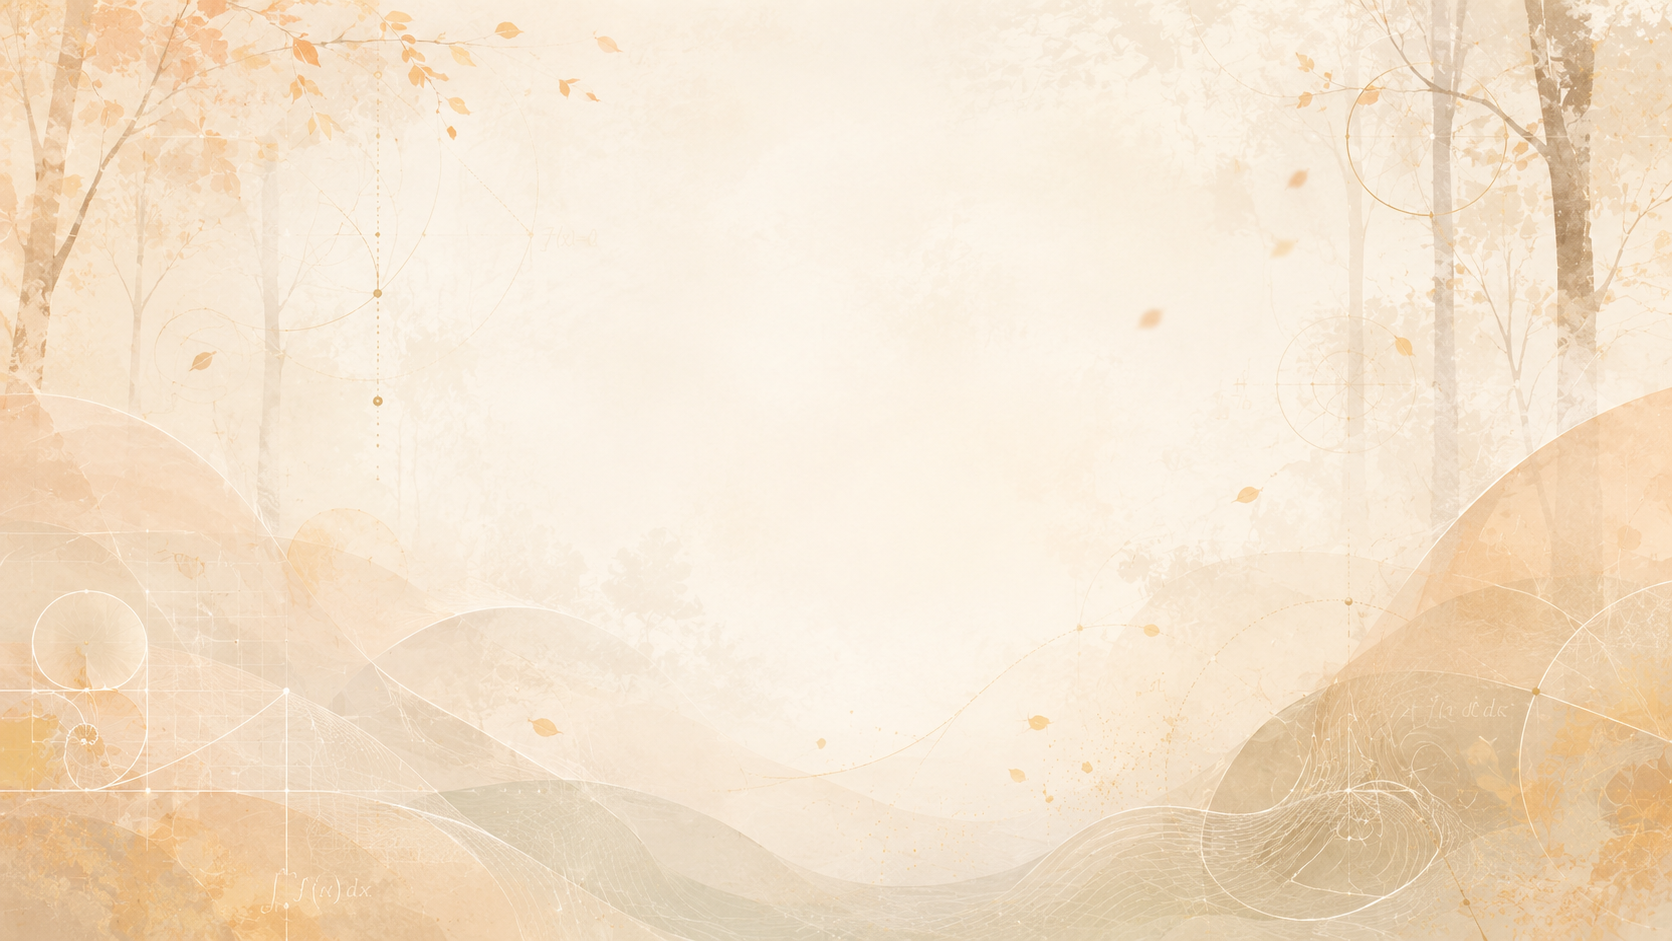
\includegraphics[width=\paperwidth,height=\paperheight,keepaspectratio=false]{chapter_04_bg_01.png}%
}
\begin{frame}[c]{Outline}
  \begin{center}
    \tableofcontents
  \end{center}
  \note{
    Here is the plan. We start with motivation: why we bother classifying
    discontinuities at all. Then we define the right-hand and left-hand
    limits of a function, the basic tool for the whole section. With those in
    hand we define the two kinds of discontinuity, the simple ones of the
    first kind and the wilder ones of the second kind. We then study four
    examples in detail, and close with a summary of what we have learned.
  }
\end{frame}

% =============================================================================
\section{Motivation}
% =============================================================================

% --- Build 1/3 ---
\begin{frame}{Why Classify Discontinuities?}
  \begin{hlbox}
  \begin{itemize}
    \item We have studied where functions \alert{are} continuous
  \end{itemize}
  \end{hlbox}

  \note{
    Up to now our whole focus has been on continuity: where a function is
    continuous, and what good behavior that guarantees. We proved that
    continuous functions preserve compactness and connectedness, and that
    they attain their maxima on compact sets. But every theorem about
    continuity invites the opposite question.
  }
\end{frame}

% --- Build 2/3 ---
\begin{frame}{Why Classify Discontinuities?}
  \begin{hlbox}
  \begin{itemize}
    \item We have studied where functions \alert{are} continuous
    \item Now: what happens where a function \alert{fails} to be continuous?
  \end{itemize}
  \end{hlbox}

  \note{
    Now we ask the reverse. Suppose a function is not continuous at some
    point. What exactly goes wrong there? A point of failure is called a
    discontinuity. As we will see, failures come in very different flavors,
    some mild and easy to describe, others genuinely chaotic.
  }
\end{frame}

% --- Build 3/3 ---
\begin{frame}{Why Classify Discontinuities?}
  \begin{hlbox}
  \begin{itemize}
    \item We have studied where functions \alert{are} continuous
    \item Now: what happens where a function \alert{fails} to be continuous?
    \item Goal: sort discontinuities into \alert{simple} vs.\ \alert{wild}
  \end{itemize}
  \end{hlbox}

  \note{
    Our goal in this section is to build a vocabulary for these failures. We
    will split discontinuities into two types: the first kind, also called
    simple discontinuities, which are tame and well understood; and the
    second kind, which are everything else. The key tool that makes this
    classification possible is the idea of a one-sided limit, so let's define
    that first.
  }
\end{frame}

% --- Recall continuity at a point ---
\begin{frame}{Recall: Continuity at a Point}
  \begin{defblock}{Definition 4.5 (recap)}
    $f$ is \alert{continuous at $x$} if $f(t) \to f(x)$ as $t \to x$;
    equivalently $\displaystyle \lim_{t \to x} f(t) = f(x)$.
  \end{defblock}

  \vspace{0.5em}
  \begin{hlbox}
  \textbf{So $f$ is \emph{discontinuous} at $x$ if this fails:} the limit
  disagrees with $f(x)$, or the limit does not exist at all.
  \end{hlbox}

  \note{
    Let's recall what continuity at a point means. A function is continuous
    at "x" if, as "t" approaches "x", the values of "f" of "t" approach "f"
    of "x". In limit notation, the limit of "f" of "t" as "t" goes to "x"
    equals "f" of "x". So a function is discontinuous at "x" precisely when
    this breaks down. Either the limit exists but does not equal the function
    value, or the limit fails to exist in the first place. To tell these
    cases apart cleanly, we need to look at the function from each side
    separately.
  }
\end{frame}

}

% =============================================================================
{
\usebackgroundtemplate{%
  
\includegraphics[width=\paperwidth,height=\paperheight,keepaspectratio=false]{chapter_04_bg_02.png}%
}
\section{One-Sided Limits}
% =============================================================================

\begin{frame}{The Idea of One-Sided Limits}
  \begin{hlbox}
  Approaching $x$ from the \alert{right} and from the \alert{left} may give
  different answers.
  \end{hlbox}

  \vspace{0.4em}
  \begin{center}
  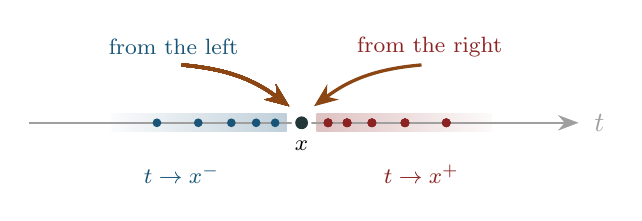
\begin{tikzpicture}[scale=1.05]
    % soft approach bands, intensifying toward x
    \shade[right color=defcolor!28, left color=defcolor!2]
      (0.7,-0.11) rectangle (2.82,0.11);
    \shade[left color=thmcolor!28, right color=thmcolor!2]
      (3.18,-0.11) rectangle (5.3,0.11);
    % axis on top of the bands
    \draw[axisln] (-0.3,0) -- (6.35,0);
    \node[gray!75] at (6.6,0) {$t$};
    % sequence points marching toward x
    \foreach \t in {1.25,1.75,2.15,2.45,2.68} \seqdot{defcolor}{(\t,0)}
    \foreach \t in {4.75,4.25,3.85,3.55,3.32} \seqdot{thmcolor}{(\t,0)}
    % curved guide arrows
    \draw[mapf] (1.55,0.7) to[bend left=16] (2.85,0.2);
    \draw[mapf] (4.45,0.7) to[bend right=16] (3.15,0.2);
    \node[defcolor, font=\footnotesize] at (1.45,0.92) {from the left};
    \node[thmcolor, font=\footnotesize] at (4.55,0.92) {from the right};
    % the point x
    \dotpt{mDarkTeal}{(3,0)}
    \node[below=3pt, font=\footnotesize] at (3,0) {$x$};
    % side labels
    \node[defcolor, font=\footnotesize] at (1.55,-0.62) {$t \to x^{-}$};
    \node[thmcolor, font=\footnotesize] at (4.45,-0.62) {$t \to x^{+}$};
  \end{tikzpicture}
  \end{center}

  \begin{hlbox}
  \textbf{Notation:} $f(x+)$ is the \alert{right-hand limit},
  $f(x-)$ the \alert{left-hand limit}.
  \end{hlbox}

  \note{
    Here is the intuition before the formal definition. On the slide you see a
    horizontal axis, labeled "t", with the point "x" marked by the dark dot in
    the center. The idea is to study the function near "x" by approaching from
    one side at a time. On the left, the blue dots march steadily rightward
    toward "x", and the shaded band deepens as they close in; the orange arrow
    points the way. As these inputs creep toward "x" from the left, the
    outputs settle on a value we call "f" of "x" minus, the left-hand limit.
    On the right, the red dots do the mirror image, and their outputs tend to
    "f" of "x" plus, the right-hand limit. Why bother splitting the approach
    in two? Because, as the labels hint, these two one-sided limits need not
    agree, and either one might fail to exist at all. That single fact is what
    the rest of the section is built on. Let's make it precise.
  }
\end{frame}

\begin{frame}{Definition 4.25: Right- and Left-Hand Limits}
  \begin{defblock}{Definition 4.25}
    Let $f$ be defined on $(a,b)$. For $a \le x < b$, write
    \[
      f(x+) = q
    \]
    if $f(t_n) \to q$ for \alert{every} sequence $\{t_n\}$ in $(x,b)$ with
    $t_n \to x$.

    \smallskip
    For $a < x \le b$, define $f(x-)$ using sequences $\{t_n\}$ in $(a,x)$.
  \end{defblock}

  \note{
    Here is the official definition. Let "f" be defined on the open interval
    from "a" to "b". For a point "x" with "a" less than or equal to "x" less
    than "b", we say "f" of "x" plus equals "q" if the following holds: take
    any sequence "t" sub "n" lying strictly to the right of "x", inside the
    interval, that converges to "x". Then the values "f" of "t" sub "n" must
    converge to "q". The word every is essential: no matter which sequence
    approaching from the right we pick, we must always land on the same limit
    "q". The left-hand limit "f" of "x" minus is defined the same way, except
    now the sequences come from the left, between "a" and "x". This is just
    the sequential definition of a limit, restricted to one side.
  }
\end{frame}

\begin{frame}{When Does the Full Limit Exist?}
  \begin{thmblock}{Key observation}
    For any $x \in (a,b)$, $\displaystyle \lim_{t \to x} f(t)$ exists
    \alert{if and only if}
    \[
      f(x+) = f(x-) = \lim_{t \to x} f(t).
    \]
  \end{thmblock}

  \vspace{0.4em}
  \begin{hlbox}
  The two-sided limit exists iff both one-sided
  limits exist \emph{and agree}.
  \end{hlbox}

  \note{
    This observation ties the one-sided limits back to the ordinary limit. At
    an interior point "x", the full two-sided limit exists if and only if
    both one-sided limits exist and are equal to each other. When that
    happens, their common value is the limit. This makes sense: approaching
    from either side has to give the same answer for a genuine limit to
    exist. This little equivalence is exactly the lens we will use to classify
    discontinuities. The whole game comes down to asking whether "f" of "x"
    plus and "f" of "x" minus exist, and whether they match each other and
    the value "f" of "x".
  }
\end{frame}

}

% =============================================================================
{
\usebackgroundtemplate{%
  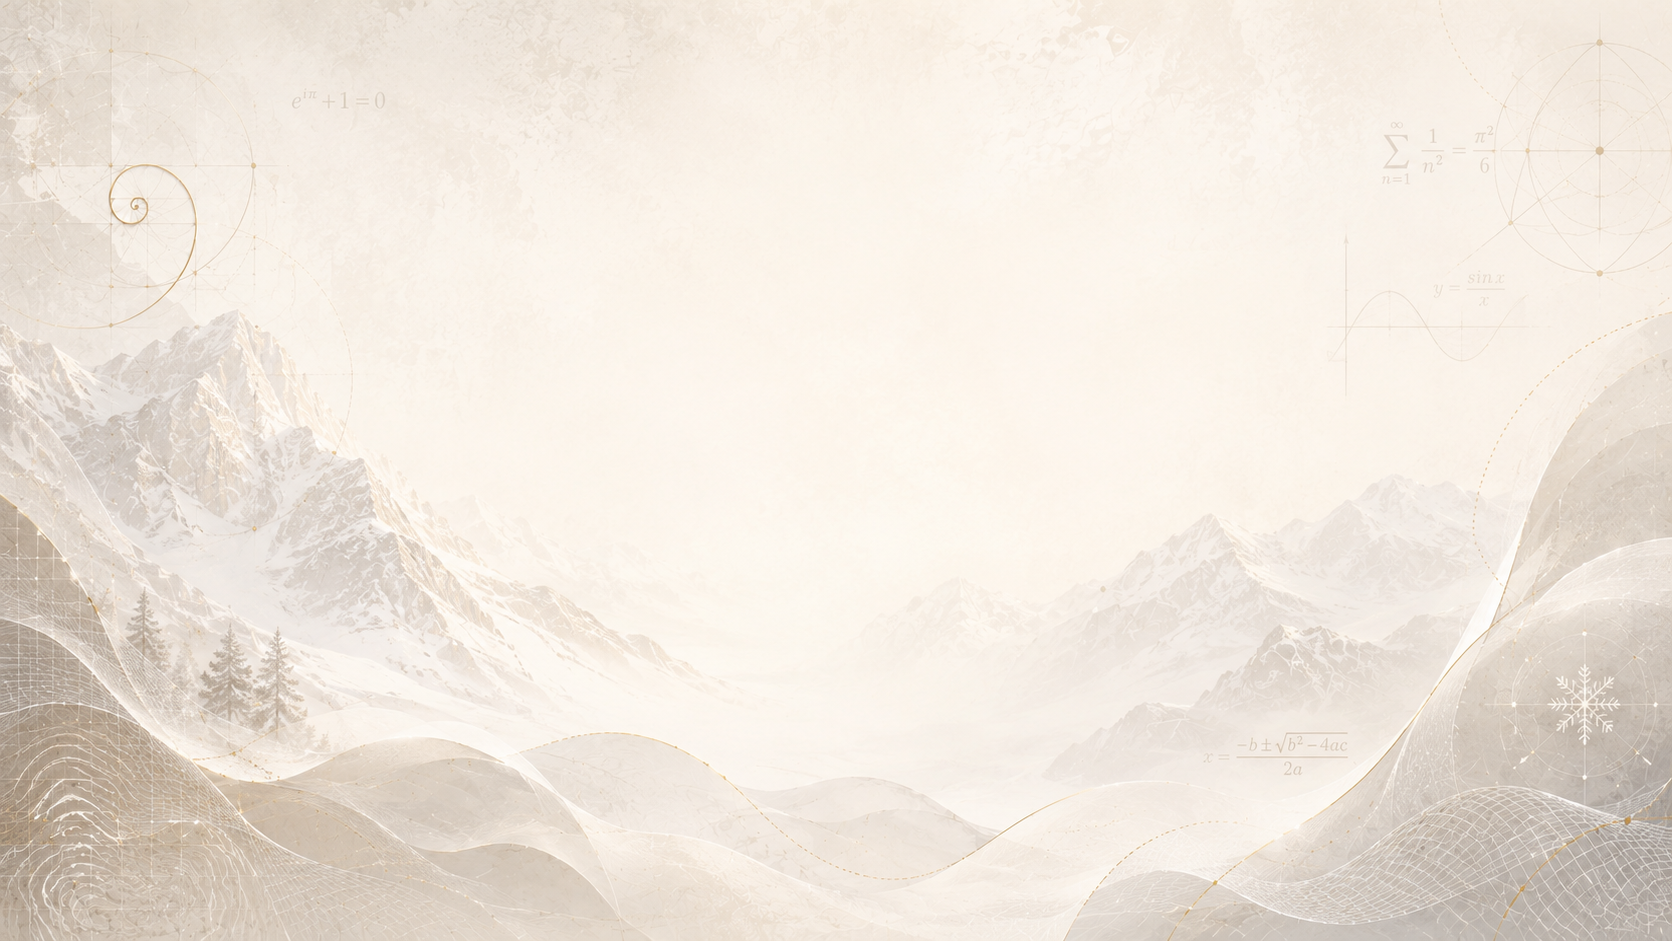
\includegraphics[width=\paperwidth,height=\paperheight,keepaspectratio=false]{chapter_04_bg_03.png}%
}
\section{Two Kinds of Discontinuity}
% =============================================================================

\begin{frame}{Definition 4.26: First and Second Kind}
  \begin{defblock}{Definition 4.26}
    Suppose $f$ is discontinuous at $x$.
    \begin{itemize}
      \item If \alert{both} $f(x+)$ and $f(x-)$ exist: discontinuity of the
        \alert{first kind}, or a \alert{simple discontinuity}.
      \item Otherwise: discontinuity of the \alert{second kind}.
    \end{itemize}
  \end{defblock}

  \vspace{0.4em}
  \begin{hlbox}
  \textbf{The dividing line:} do both one-sided limits exist?
  \end{hlbox}

  \note{
    Now the central definition of the section. Suppose "f" is discontinuous
    at a point "x". We split into two cases based on a single question: do
    both one-sided limits exist? If both "f" of "x" plus and "f" of "x" minus
    exist as honest numbers, we call this a discontinuity of the first kind,
    or a simple discontinuity. If at least one of the one-sided limits fails
    to exist, it is a discontinuity of the second kind. So the entire
    classification hinges on the existence of those two one-sided limits, not
    on their values. Let's see what the simple case can look like.
  }
\end{frame}

\begin{frame}{Two Flavors of Simple Discontinuity}
  \begin{hlbox}
  Both $f(x+)$ and $f(x-)$ exist, yet $f$ is still discontinuous. Two ways:
  \begin{enumerate}
    \item[(1)] $f(x+) \neq f(x-)$ \quad ---\quad a \alert{jump}
      (the value $f(x)$ is irrelevant).
    \item[(2)] $f(x+) = f(x-) \neq f(x)$ \quad ---\quad a \alert{removable}
      discontinuity.
  \end{enumerate}
  \end{hlbox}

  \vspace{0.6em}
  \begin{center}
  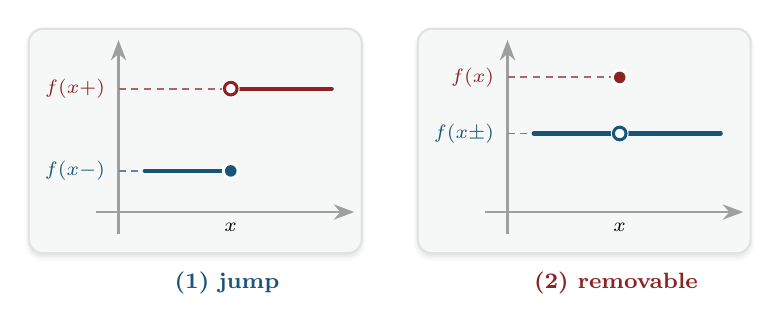
\begin{tikzpicture}[scale=0.95]
    % --- Jump (left picture) ---
    \begin{scope}[xshift=0cm]
      \draw[panel] (-1.2,-0.55) rectangle (3.25,2.45);
      \draw[axisln] (-0.3,0) -- (3.15,0);
      \draw[axisln] (0,-0.3) -- (0,2.3);
      % projection lines to the y-axis
      \draw[projln, defcolor!70] (0,0.55) -- (1.5,0.55);
      \draw[projln, thmcolor!70] (0,1.65) -- (1.5,1.65);
      \node[defcolor, left, font=\scriptsize] at (-0.05,0.55) {$f(x{-})$};
      \node[thmcolor, left, font=\scriptsize] at (-0.05,1.65) {$f(x{+})$};
      % graph
      \draw[curveln, defcolor] (0.35,0.55) -- (1.5,0.55);
      \draw[curveln, thmcolor] (1.5,1.65) -- (2.85,1.65);
      \opendot{thmcolor}{(1.5,1.65)}
      \dotpt{defcolor}{(1.5,0.55)}
      \node[below, font=\scriptsize] at (1.5,-0.02) {$x$};
      \node[font=\footnotesize\bfseries, defcolor] at (1.45,-0.95) {(1) jump};
    \end{scope}
    % --- Removable (right picture) ---
    \begin{scope}[xshift=5.2cm]
      \draw[panel] (-1.2,-0.55) rectangle (3.25,2.45);
      \draw[axisln] (-0.3,0) -- (3.15,0);
      \draw[axisln] (0,-0.3) -- (0,2.3);
      % projection lines to the y-axis
      \draw[projln, defcolor!70] (0,1.05) -- (1.5,1.05);
      \draw[projln, thmcolor!70] (0,1.8) -- (1.5,1.8);
      \node[defcolor, left, font=\scriptsize] at (-0.05,1.05) {$f(x{\pm})$};
      \node[thmcolor, left, font=\scriptsize] at (-0.05,1.8) {$f(x)$};
      % graph
      \draw[curveln, defcolor] (0.35,1.05) -- (2.85,1.05);
      \opendot{defcolor}{(1.5,1.05)}
      \dotpt{thmcolor}{(1.5,1.8)}
      \node[below, font=\scriptsize] at (1.5,-0.02) {$x$};
      \node[font=\footnotesize\bfseries, thmcolor] at (1.45,-0.95) {(2) removable};
    \end{scope}
  \end{tikzpicture}
  \end{center}

  \note{
    When both one-sided limits exist, there are exactly two ways the function
    can still be discontinuous. The first is a jump, shown in the left panel.
    The graph sits at one height coming from the left, the solid blue dot,
    then leaps to a different height on the right, the open red dot. The dashed
    lines carry each of these heights across to the vertical axis, where they
    are labeled "f" of "x" minus and "f" of "x" plus, so you can see at a
    glance that the two sides land in different places. For a jump, the actual
    value "f" of "x" does not matter at all; the mismatch of the two sides
    already forces the discontinuity. The second flavor is a removable
    discontinuity, in the right panel. Here both sides agree, the graph
    approaches one common height from both directions, marked by the open dot,
    but the function value itself, the solid dot floating above it, sits
    somewhere else. It is called removable because you could repair it in a
    single stroke, just redefine "f" of "x" to be that common limit and the
    function becomes continuous. Both of these are discontinuities of the
    first kind.
  }
\end{frame}

\begin{frame}{The Full Taxonomy}
  \begin{center}
  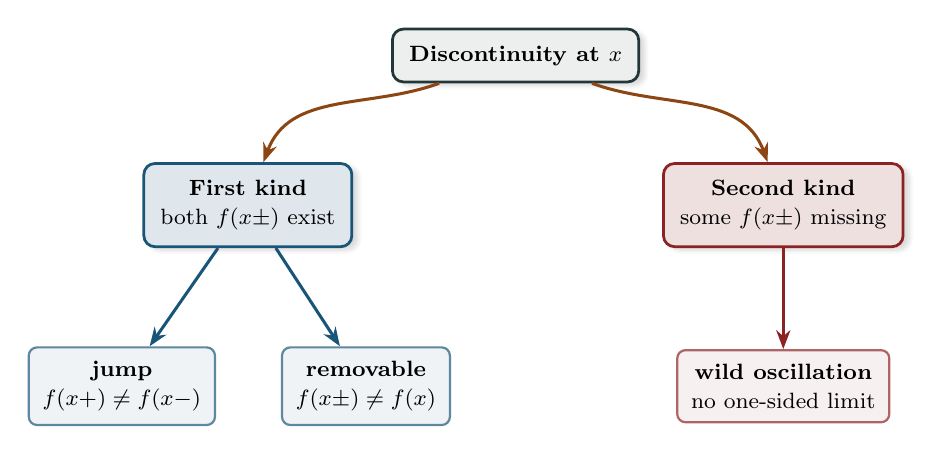
\begin{tikzpicture}[scale=1.0, font=\footnotesize,
      box/.style={rounded corners=4pt, line width=1pt, inner sep=6pt, align=center,
        blur shadow={shadow blur steps=7, shadow opacity=16, shadow yshift=-1.2pt}},
      leaf/.style={rounded corners=3pt, line width=0.8pt, inner sep=5pt, align=center},
      edge/.style={line width=1.1pt, -{Stealth[length=2.4mm]}, rounded corners}]
    \node[box, draw=mDarkTeal, fill=mDarkTeal!8] (top)
      at (0,3.0) {\textbf{Discontinuity at $x$}};
    \node[box, draw=defcolor, fill=defcolor!14] (first)
      at (-3.4,1.1) {\textbf{First kind}\\[1pt]\footnotesize both $f(x\pm)$ exist};
    \node[box, draw=thmcolor, fill=thmcolor!14] (second)
      at (3.4,1.1) {\textbf{Second kind}\\[1pt]\footnotesize some $f(x\pm)$ missing};
    \node[leaf, draw=defcolor!70, fill=defcolor!7] (jump) at (-5.0,-1.2)
      {\textbf{jump}\\[1pt]$f(x+)\neq f(x-)$};
    \node[leaf, draw=defcolor!70, fill=defcolor!7] (rem) at (-1.9,-1.2)
      {\textbf{removable}\\[1pt]$f(x\pm)\neq f(x)$};
    \node[leaf, draw=thmcolor!70, fill=thmcolor!7] (wild) at (3.4,-1.2)
      {\textbf{wild oscillation}\\[1pt]no one-sided limit};
    \draw[edge, mAccent] (top) to[out=200,in=70] (first);
    \draw[edge, mAccent] (top) to[out=-20,in=110] (second);
    \draw[edge, defcolor] (first) -- (jump);
    \draw[edge, defcolor] (first) -- (rem);
    \draw[edge, thmcolor] (second) -- (wild);
  \end{tikzpicture}
  \end{center}

  \note{
    Let's gather the whole classification into one tree. At the top sits the
    starting point, a discontinuity at some "x". It immediately forks into two
    branches. The blue branch on the left is the first kind, the simple
    discontinuities, defined by the condition that both one-sided limits exist.
    It in turn splits into the two leaves we just studied: a jump, where the
    two sides disagree, and a removable discontinuity, where the two sides
    agree but differ from the function value. The red branch on the right is
    the second kind, where at least one one-sided limit is missing; its leaf is
    labeled wild oscillation, the behavior we will meet in a moment. Notice the
    whole tree is driven by just one yes-or-no question at each fork, so the
    scheme is genuinely simple. Keep this map in mind, because the four
    examples coming up are nothing more than instances sitting at its various
    leaves.
  }
\end{frame}

}

% =============================================================================
{
\usebackgroundtemplate{%
  
\includegraphics[width=\paperwidth,height=\paperheight,keepaspectratio=false]{chapter_04_bg_04.png}%
}
\section{Examples}
% =============================================================================

\begin{frame}{Example 4.27(a): The Dirichlet Function}
  \begin{exblock}{Example 4.27(a)}
    \[
      f(x) = \begin{cases} 1 & (x \text{ rational}), \\ 0 & (x \text{ irrational}). \end{cases}
    \]
    At \alert{every} point, neither $f(x+)$ nor $f(x-)$ exists
    $\;\Rightarrow\;$ discontinuity of the \alert{second kind} everywhere.
  \end{exblock}

  \note{
    Our first example is the famous Dirichlet function. It equals one at
    every rational number and zero at every irrational number. Now ask for a
    one-sided limit at any point. As we approach from the right, we keep
    hitting both rationals and irrationals arbitrarily close together, so the
    values keep bouncing between one and zero and never settle. That means
    "f" of "x" plus simply does not exist, and the same goes for "f" of "x"
    minus. Since the one-sided limits fail to exist, this is a discontinuity
    of the second kind, and it happens at every single point of the real
    line. A maximally bad discontinuity.
  }
\end{frame}

\begin{frame}{Example 4.27(b): A Single Point of Rescue}
  \begin{exblock}{Example 4.27(b)}
    \[
      f(x) = \begin{cases} x & (x \text{ rational}), \\ 0 & (x \text{ irrational}). \end{cases}
    \]
    \alert{Continuous at $x = 0$}; discontinuity of the \alert{second kind}
    at every other point.
  \end{exblock}

  \vspace{0.3em}
  \begin{hlbox}
  \textbf{Why $x=0$ works:} near $0$, both branches ($x$ and $0$) are tiny,
  so $f(t) \to 0 = f(0)$.
  \end{hlbox}

  \note{
    The second example is a clever variation. Now "f" of "x" equals "x" when
    "x" is rational and zero when "x" is irrational. Consider the point zero.
    As "t" approaches zero, the rational branch gives "t", which goes to
    zero, and the irrational branch gives zero outright. So both kinds of
    points produce values heading to zero, which is exactly "f" of zero.
    Hence "f" is continuous at zero. But at any other point "p", the rational
    values cluster near "p" while the irrational values stay at zero, so the
    function again oscillates and the one-sided limits fail to exist. Every
    point except zero is a discontinuity of the second kind. One single point
    of continuity in a sea of chaos.
  }
\end{frame}

\begin{frame}{Example 4.27(c): A Genuine Jump}
  \begin{exblock}{Example 4.27(c)}
    \[
      f(x) = \begin{cases} x + 2 & (-3 < x < -2), \\ -x - 2 & (-2 \le x < 0), \\ x + 2 & (0 \le x < 1). \end{cases}
    \]
    \alert{Simple discontinuity} at $x=0$; continuous elsewhere on $(-3,1)$.
  \end{exblock}

  \note{
    The third example is concrete and piecewise. On the first piece "f" of
    "x" is "x" plus two, on the middle piece it is minus "x" minus two, and
    on the last piece it is again "x" plus two. Let's check the point zero,
    which is where the middle and last pieces meet. Coming from the left we
    use minus "x" minus two, which approaches minus two as "x" goes to zero.
    Coming from the right, and at zero itself, we use "x" plus two, which
    gives two. So the left-hand limit is minus two and the right-hand limit
    is two: both exist but disagree. That is a jump, a simple discontinuity
    of the first kind. Everywhere else the formula is continuous. Let's see
    the graph.
  }
\end{frame}

\begin{frame}{Example 4.27(c): The Graph}
  \begin{center}
  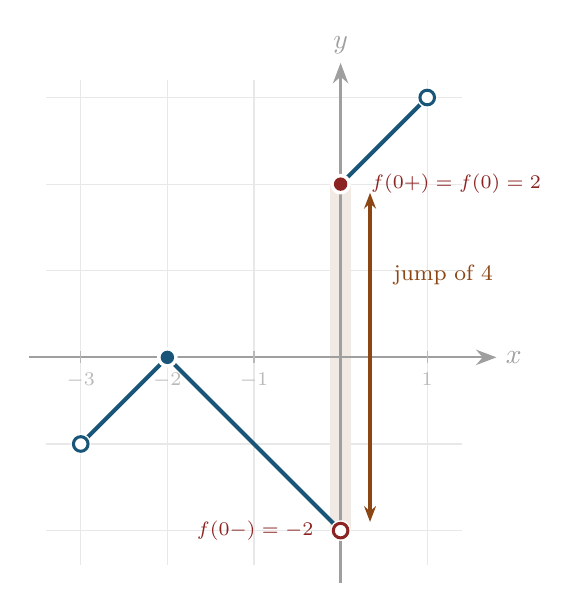
\begin{tikzpicture}[scale=1.1]
    % faint reference grid
    \draw[gray!18, line width=0.4pt, ystep=1, xstep=1] (-3.4,-2.4) grid (1.4,3.2);
    % shaded jump band at x=0
    \fill[mAccent!12] (-0.12,-2) rectangle (0.12,2);
    \draw[axisln] (-3.6,0) -- (1.8,0); \node[gray!75] at (2.0,0) {$x$};
    \draw[axisln] (0,-2.6) -- (0,3.4); \node[gray!75] at (0,3.6) {$y$};
    \foreach \x in {-3,-2,-1,1} \draw[gray!55] (\x,0.07) -- (\x,-0.07) node[below, font=\scriptsize]{$\x$};
    \foreach \y in {-2,2} \draw[gray!55] (0.07,\y) -- (-0.07,\y);
    % projection lines to the one-sided limits
    \draw[projln, thmcolor!65] (0,-2) -- (-0.12,-2);
    \draw[projln, thmcolor!65] (0,2) -- (0.12,2);
    % piece 1: x+2 on (-3,-2): from (-3,-1) to (-2,0)
    \draw[curveln, defcolor] (-3,-1) -- (-2,0);
    \opendot{defcolor}{(-3,-1)}
    % piece 2: -x-2 on [-2,0): from (-2,0) to (0,-2)
    \draw[curveln, defcolor] (-2,0) -- (0,-2);
    \dotpt{defcolor}{(-2,0)}
    \opendot{thmcolor}{(0,-2)}
    % piece 3: x+2 on [0,1): from (0,2) to (1,3)
    \draw[curveln, defcolor] (0,2) -- (1,3);
    \dotpt{thmcolor}{(0,2)}
    \opendot{defcolor}{(1,3)}
    % annotate the jump
    \draw[mapf, {Stealth[length=2mm]}-{Stealth[length=2mm]}] (0.34,-1.9) -- (0.34,1.9);
    \node[mAccent, right, font=\footnotesize] at (0.5,0.95) {jump of $4$};
    \node[thmcolor, left, font=\scriptsize] at (-0.2,-2) {$f(0-)=-2$};
    \node[thmcolor, right, font=\scriptsize] at (0.24,2.00) {$f(0+)=f(0)=2$};
  \end{tikzpicture}
  \end{center}

  \note{
    Here is the picture. Reading left to right: the first two pieces connect
    smoothly, forming a peak at "x" equals minus two with no break there,
    that corner is still continuous. Then watch what happens at "x" equals
    zero. The graph slides down to the open red dot at height minus two, the
    left-hand limit. But the next piece starts up at the solid dot at height
    two, which is both the right-hand limit and the actual value "f" of zero.
    The burnt-orange double arrow marks the size of the jump, a gap of four
    units. Both one-sided limits exist, they just refuse to meet. This is the
    cleanest possible example of a simple jump discontinuity.
  }
\end{frame}

\begin{frame}{Example 4.27(d): Wild Oscillation}
  \begin{exblock}{Example 4.27(d)}
    \[
      f(x) = \begin{cases} \sin \dfrac{1}{x} & (x \neq 0), \\[6pt] 0 & (x = 0). \end{cases}
    \]
    Neither $f(0+)$ nor $f(0-)$ exists $\;\Rightarrow\;$ discontinuity of the
    \alert{second kind} at $0$; continuous for $x \neq 0$.
  \end{exblock}

  \note{
    Our last example is sine of one over "x", with the value patched to be
    zero at the origin. As "x" gets close to zero, one over "x" races off to
    infinity, so the sine oscillates faster and faster between minus one and
    one, infinitely many times in any tiny interval around zero. The values
    never approach any single number, so neither the right-hand nor the
    left-hand limit exists. That makes zero a discontinuity of the second
    kind. Away from zero, sine of one over "x" is a composition of continuous
    functions, so by the composition theorem, Theorem 4.7, it is continuous
    everywhere else. Let's look at how dramatic this is.
  }
\end{frame}

\begin{frame}{Example 4.27(d): The Graph}
  \begin{center}
  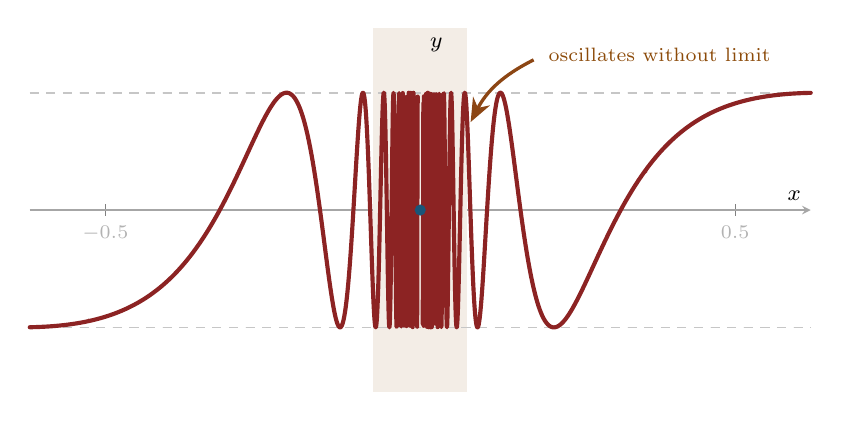
\begin{tikzpicture}
    \begin{axis}[
      width=11.5cm, height=6.2cm,
      axis lines=middle,
      axis line style={gray!70},
      xlabel={\footnotesize $x$}, ylabel={\footnotesize $y$},
      xmin=-0.62, xmax=0.62, ymin=-1.55, ymax=1.55,
      ytick={-1,1}, xtick={-0.5,0.5},
      tick label style={font=\scriptsize, gray!60},
      clip=false,
      samples=2000, domain=0.004:0.62,
    ]
      % highlighted "wild zone" near the origin
      \fill[excolor!10] (axis cs:-0.075,-1.55) rectangle (axis cs:0.075,1.55);
      % envelope lines y = +/- 1
      \addplot[dashed, gray!45, line width=0.6pt, domain=-0.62:0.62] {1};
      \addplot[dashed, gray!45, line width=0.6pt, domain=-0.62:0.62] {-1};
      % the curve
      \addplot[curveln, thmcolor] {sin(deg(1/x))};
      \addplot[curveln, thmcolor, domain=-0.62:-0.004] {sin(deg(1/x))};
      % patched value at the origin
      \addplot[only marks, mark=*, mark size=1.8pt, defcolor] coordinates {(0,0)};
      % annotation
      \node[excolor, font=\scriptsize, align=center] at (axis cs:0.38,1.32)
        {oscillates without limit};
      \draw[mapf] (axis cs:0.18,1.28) to[bend right=18] (axis cs:0.08,0.75);
    \end{axis}
  \end{tikzpicture}
  \end{center}

  \note{
    And here is the graph. As you move toward the center from either side, the
    red curve compresses into an ever denser band of oscillations, sweeping
    between the two dashed lines at height one and height minus one without
    ever resting. Those dashed lines are the envelope, the band the sine can
    never leave. The shaded strip down the middle marks the trouble zone right
    around zero; no matter how far you zoom into it, the picture looks just as
    busy, because the curve crosses every height between minus one and one
    infinitely often there. The blue dot at the origin is our patched value of
    zero, but the curve around it never settles toward any single height, so
    that dot is not the limit of anything. This is the visual signature of a
    second-kind discontinuity: not a jump, not a hole, but genuine refusal to
    converge. It is a striking contrast to the clean jump of the previous
    example.
  }
\end{frame}

}

% =============================================================================
{
\usebackgroundtemplate{%
  
\includegraphics[width=\paperwidth,height=\paperheight,keepaspectratio=false]{chapter_04_bg_05.png}%
}
\section{Summary}
% =============================================================================

% --- Build 1/4 ---
\begin{frame}{Summary}
  \begin{hlbox}
  \textbf{Key takeaways:}
  \begin{itemize}
    \item \alert{One-sided limits} $f(x+)$, $f(x-)$: approach $x$ from one side.
  \end{itemize}
  \end{hlbox}

  \note{
    Let's gather what we learned. The fundamental tool of this section is the
    one-sided limit. The right-hand limit "f" of "x" plus and the left-hand
    limit "f" of "x" minus describe how the function behaves as we approach
    "x" purely from the right or purely from the left. Everything else was
    built on these.
  }
\end{frame}

% --- Build 2/4 ---
\begin{frame}{Summary}
  \begin{hlbox}
  \textbf{Key takeaways:}
  \begin{itemize}
    \item \alert{One-sided limits} $f(x+)$, $f(x-)$: approach $x$ from one side.
    \item \alert{First kind} (simple): both one-sided limits exist
      --- a jump or a removable hole.
  \end{itemize}
  \end{hlbox}

  \note{
    Using one-sided limits, we classified discontinuities. A discontinuity of
    the first kind, also called simple, is one where both one-sided limits
    exist. It comes in two shapes: a jump, where the two sides disagree, and
    a removable discontinuity, where the two sides agree but differ from the
    function value. These are the tame, well-behaved failures.
  }
\end{frame}

% --- Build 3/4 ---
\begin{frame}{Summary}
  \begin{hlbox}
  \textbf{Key takeaways:}
  \begin{itemize}
    \item \alert{One-sided limits} $f(x+)$, $f(x-)$: approach $x$ from one side.
    \item \alert{First kind} (simple): both one-sided limits exist
      --- a jump or a removable hole.
    \item \alert{Second kind}: at least one one-sided limit fails to exist.
  \end{itemize}
  \end{hlbox}

  \note{
    Everything else is a discontinuity of the second kind: at least one of
    the one-sided limits fails to exist. The Dirichlet function and sine of
    one over "x" gave us vivid pictures of this, oscillation so violent that
    no one-sided limit can form. These are the wild discontinuities.
  }
\end{frame}

% --- Build 4/4 ---
\begin{frame}{Summary}
  \begin{hlbox}
  \textbf{Key takeaways:}
  \begin{itemize}
    \item \alert{One-sided limits} $f(x+)$, $f(x-)$: approach $x$ from one side.
    \item \alert{First kind} (simple): both one-sided limits exist
      --- a jump or a removable hole.
    \item \alert{Second kind}: at least one one-sided limit fails to exist.
  \end{itemize}

  \vspace{0.8em}
  \textbf{Coming up next:} \emph{Monotonic Functions} --- where simple
  discontinuities are the \alert{only} kind possible.
  \end{hlbox}

  \note{
    With this vocabulary in place, we are ready for the next section on
    monotonic functions. There we will prove a remarkable fact: a monotonic
    function can only have discontinuities of the first kind, the simple
    jumps, and moreover it can have at most countably many of them. The wild
    second-kind behavior we saw today is simply impossible once a function is
    monotonic. That is a perfect illustration of how today's classification
    pays off. See you in the next section.
  }
\end{frame}
}

\end{document}
